%-------------------------------------------------------------------------------
\chapter[Introduction]{Introduction}
%-------------------------------------------------------------------------------

%-------------------------------------------------------------------------------
\section{Preliminaries}
%-------------------------------------------------------------------------------
\gaia{} is the brand new open-source, sediment transport and bed evolution module of the \telemacsystem{} modelling system. \gaia{} is based on the historical sediment transport module \sisyphe{}, where a large number of improvements, corrections and optimizations have been implemented. Thanks to its unified framework, \gaia{} efficiently manages different sediment classes, sand-mud mixtures, etc. for both 2D and 3D spatial dimensions.

The module \sisyphe{} of the \telemacsystem{} modelling system (\textsc{TMS}) has been developed for more than 25 years~\cite{Sisyphe1.0}, originally based on the same finite element structure as the two-dimensional code solving the shallow water equations. This shallow water code later evolved into a module that was baptized \telemac{2D}.

Despite its robustness, flexibility and capability of dealing with a large number of river~\cite{ctccrp19,dwtg17}, coastal~\cite{BROWN20091502,ROBINS2014311,10.2307/40928823}, and estuarine~\cite{sfth,sfth17,doi:10.1061/(ASCE)0733-950X(2009)135:4(176)} sediment transport and morphodynamics problems~\cite{VILLARET2013105}, as well as the tremendous effort to deliver a module able to be used in both industrial and scientific contexts, a number of issues arose regarding the improvement of the treatment of graded and mixed (cohesive and non-cohesive) sediments, as well as the full compatibility between 2D and 3D processes.

From early discussions starting \textit{circa} 2014 following the developments on mixed sediment implemented \textit{ad hoc} by a consortium member for an estuarine model~\cite{deLinares}, going through strategic meetings, animated coffee debates and \textit{hackathons} involving several members of the \textsc{Telemac-Mascaret} consortium, and more recently the participation of final users and an increasing number of threads with suggestions and recommendations posted in the \textsc{TMS}'s webpage forum, the brand new sediment transport and bed evolution module \gaia{} of the \textsc{TMS} is introduced.

\gaia{}, building upon the \sisyphe{} module, is able to model complex sediment and morphodynamic processes in coastal areas, rivers, lakes and estuaries, accounting for spatial and temporal variability of sediment size classes (uniform, graded or mixed), properties (cohesive and non-cohesive) and transport modes (suspended, bedload and both simultaneously). \textbf{The generalized framework used for bed layering enables any combination of multiple size classes for both non-cohesive and cohesive sediment to be modelled simultaneously.} Compatibility is ensured between an active layer model (an approach traditionally adopted for non-cohesive sediment) and the presence of different classes of fine sediment and consolidation. \textbf{In contrast to \sisyphe{}, the quantity of each sediment class in the bed is evaluated using dry mass instead of volume, which minimizes roundoff errors.}

Although invisible to the end user, suspended sediment transport processes are dealt with by the hydrodynamic modules (\telemac{2D} or \telemac{3D}), while near-bed, bedload and processes in the bottom layer are handled by \gaia{}. This allows a clearer treatment of sedimentary processes that happen in the water column, in the bed structure and at the water-bed interface, see Figure~\ref{fig:sketch}. \gaia{} can also be coupled with the modules for sediment dredging \textsc{Nestor}, wave propagation \tomawac{} and water quality \textsc{Waqtel}.

\gaia{} can easily be expanded and customized to particular requirements by modifying friendly,
easy to read Fortran files. An overview of different applications of \gaia{} can be consulted in the yearly-published Telemac-Mascaret User Conference proceedings, freely available at the website \texttt{www.opentelemac.org}.

\begin{figure}
\centering
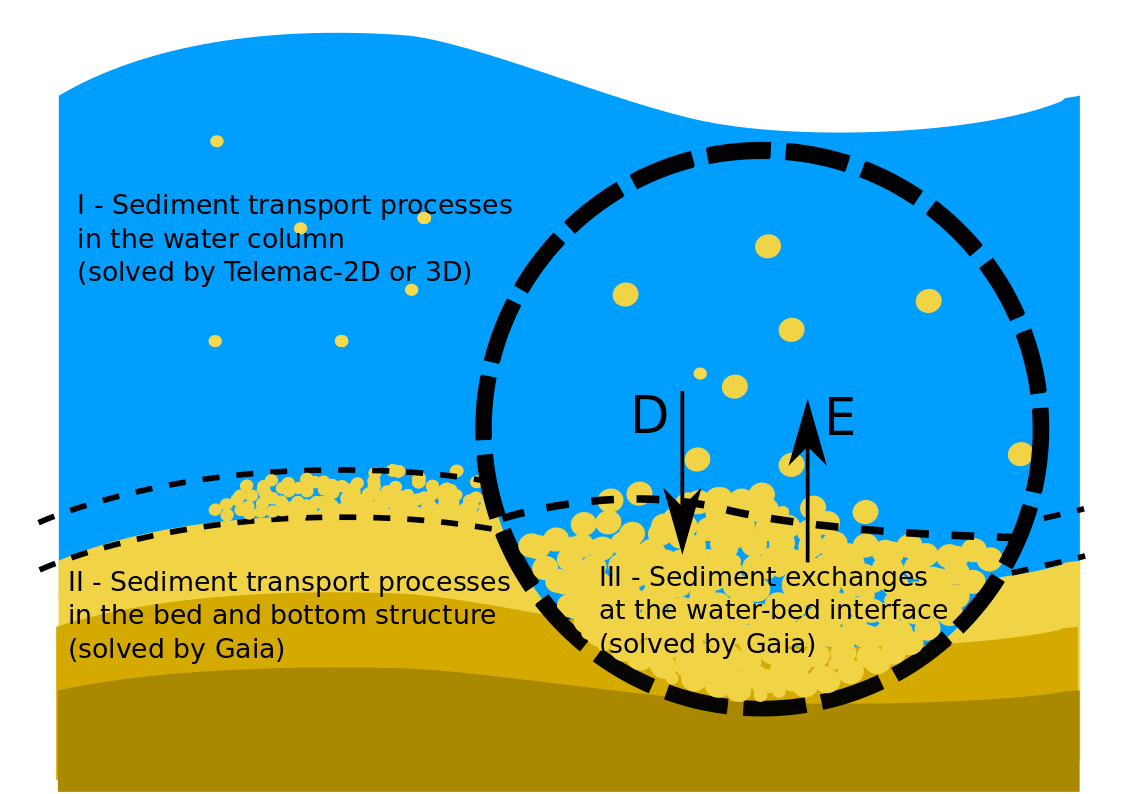
\includegraphics[trim=0 0 0 0, clip,scale=0.22]{./graphics/sediment_transport_processes}
\caption{Sketch summarizing the way in which the sediment transport mechanisms are dealt in \gaia{}. Above, $D$ and $E$ stand for deposition and entrainment fluxes.}
\label{fig:sketch}
\end{figure}


%-------------------------------------------------------------------------------
\subsection{Sediment transport and morphodynamic modelling}
%-------------------------------------------------------------------------------
The prediction of topography changes and sediment discharges can be performed by integrating several modules. It is a {\bf multi--scale problem}, with different physical mechanisms acting according to their space and time response. In summary, the relevant mechanisms that drives morphological changes are:
\begin{itemize}
         \item {\bf hydrodynamics:} with conservative laws of mass and momentum,
         \item {\bf sediment transport:} with predictors for sediment transport capacity,
         \item {\bf bed evolution:} with conservative law for sediment mass.
\end{itemize}
\noindent
Such a modelling system is often referred to as a \emph{morphodynamic model} and is the one adopted in the \telemacsystem{}.

\noindent
From the literature, the main mechanisms of sediment transport are classified as:
\begin{itemize}
\item \textcolor{black}{\bf bedload:} with a variety of closure relationships for sediment transport capacity,
\item \textcolor{black}{\bf suspended load:} with the solution of the advection-diffusion equation (ADE) plus closures for erosion and deposition fluxes, equilibrium concentration,
\item \textcolor{black}{\bf bed evolution:} with the solution of the sediment mass conservation equation or \textit{Exner equation}.
\end{itemize}

\noindent
Different types of sediment can be classified as:
\begin{itemize}
\item \textcolor{black}{\bf non-cohesive:} with equilibrium formulas
\item \textcolor{black}{\bf cohesive:} erosion and deposition laws, consolidation models
\item \textcolor{black}{\bf mixed-size sediments:} accounting for moderately or poorly sorted sediment distribution, sand-gravel and sand-mud mixtures.
\end{itemize}
\noindent


%-------------------------------------------------------------------------------
\subsection{Choice of hydrodynamic models for sediment transport applications}
%-------------------------------------------------------------------------------
The choice of appropriate model equations for flow and sediment transport
will depend upon the scales of interest.

At the scale of ripples, the mechanics of sediment transport could be coupled with the
Reynolds--averaged Navier Stokes equations (NS) to describe the phenomenon.
At large scales, however, the shallow water equations (SWE) are known to
capture quite accurately the salient features --in an average sense-- of
water bodies. The SWE are derived by simplifying the hydrodynamics in the vertical
direction instead of using the full three--dimensional NS or Euler
equations.

As such, the SWE are obtained by assuming a hydrostatic pressure
distribution and a uniform velocity profile across the water layer,
resulting in a two--dimensional problem where the primary variables are the
vertical averages of the horizontal flow velocities and water depth.

This simplification enhances the speed of computations and
facilitates further analytical approaches. In brief, the SWE are often
used to model advection--dominated open channel flows, river and lake
hydrodynamics, floodplain flows, estuarine and coastal circulation as well
as long wave run-up and hydraulic bores, among
other problems of interest within the engineering community~\cite{Vreugdenhil:94}.

%\gaia{} can be coupled with the SWE solver \telemac{2D} and the NS solver \telemac{3D} (see \S\ref{ch:3DBedloadTransport}).

%-------------------------------------------------------------------------------
\subsection{Coupling hydrodynamics to morphodynamics}
%-------------------------------------------------------------------------------
Morphological models can be run fully coupled~\cite{cao02} and decoupled~\cite{vriend87}. In a fully coupled model, sediment
transport and flow occur simultaneously, and thus, their respective
equations are coupled and should be solved simultaneously. Rapid morphological evolution processes due
to hyper-concentrated sediment--laden floods, and debris flow are typical
examples were the fully coupled approach must be employed~\cite{Frac02}.

In contrast, decoupled models are applicable when the typical time scale for river or sea bed adjustment
is much longer than the typical time scale for water flow. The approach used by \gaia{} follows the decoupled treatment, i.e., to alternate between the simulation of flow and bed evolution. This procedure, also known as \textit{asynchronous} solution, considers that the bottom is fixed when the flow variables are computed by the hydrodynamics module.

Hydrodynamic solution is therefore to solve the hydrodynamic continuity and momentum equations on a short time scale.
During this hydrodynamic step the bottom is frozen and the discretized sediment equation is subsequently solved separately.
For the current version of \gaia{}, the decoupled approach is implemented.


\begin{figure}[H]%
\begin{center}
%
\hfil
%
\subfloat[currents only]{
  %
  \vspace{-1cm}
  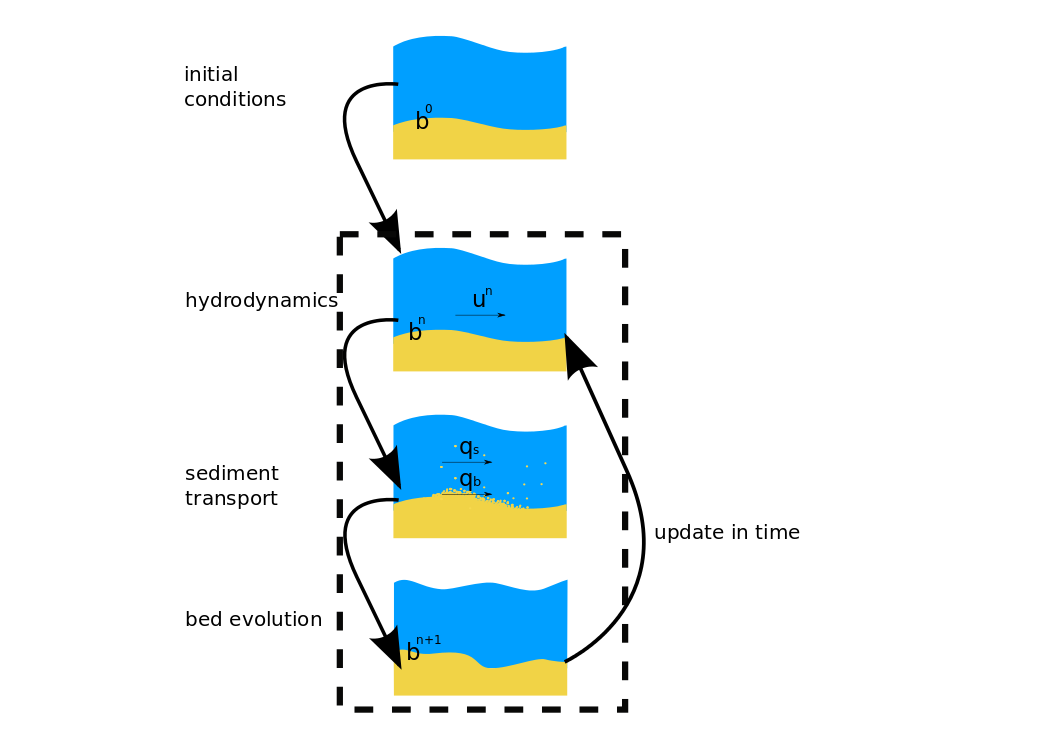
\includegraphics[width=0.55\textwidth]{./graphics/2waycoupling.png}
%
}
%
\hfil
%
\subfloat[currents $+$ waves]{
%
  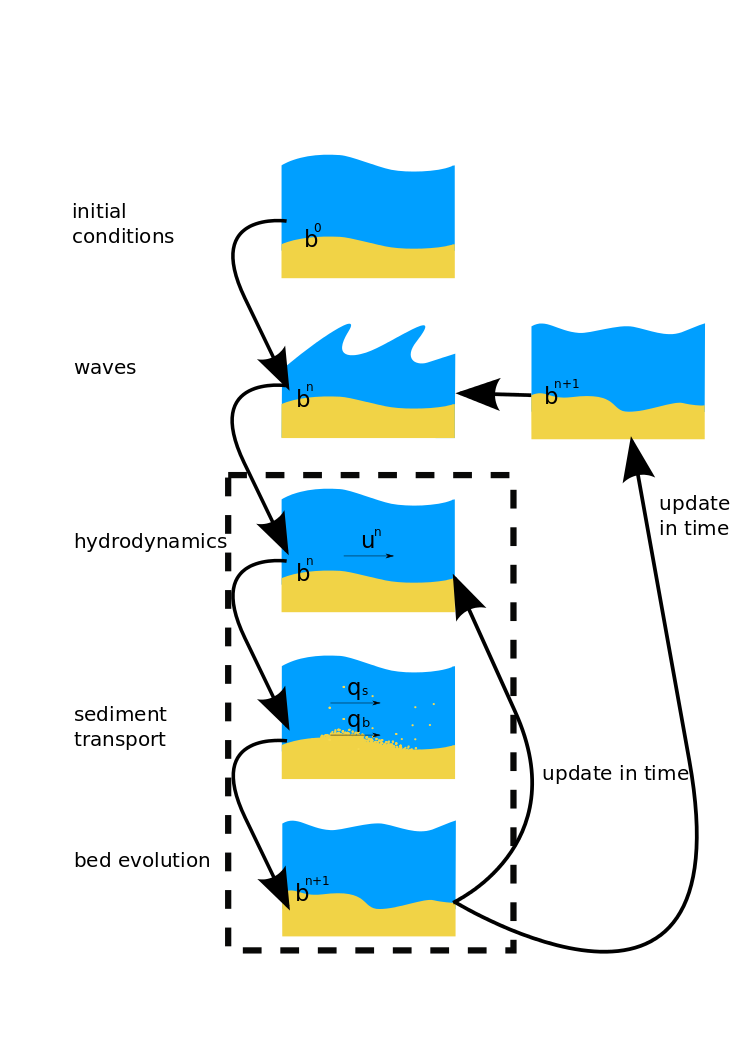
\includegraphics[width=0.4\textwidth]{./graphics/3waycoupling.png}
%
}
%
\hfil
\mbox{}
\end{center}
\caption
[Coupling strategies]
{Schematic coupling strategies for \gaia: (a) coupling morphodynamic and hydrodynamic, current only, (b) coupling morphodynamic and hydrodynamic including the effect of waves.}
\label{fig:CouplingStrategies}
\end{figure}

\pagebreak

%-------------------------------------------------------------------------------
\section{\gaia{}'s structure}
%-------------------------------------------------------------------------------

%...............................................................................
\subsection{Coupling hydrodynamics and morphodynamics}
%...............................................................................
\gaia{} can be internally coupled with the hydrodynamic models \telemac{2D} or \telemac{3D}. In the \telemac{2D} or \telemac{3D} steering files, the following keywords need to be specified:
\begin{itemize}
\item \telkey{COUPLING WITH = 'GAIA'}
\item \telkey{GAIA STEERING FILE = '<name of the gaia steering file>'}
\end{itemize}
For a \textit{hotstart} from a fully developed hydrodynamic, the following information must be included in the \telemac{2D} or \telemac{3D} steering files:
\begin{itemize}
\item \telkey{COMPUTATION CONTINUED} (logical type, set to {\ttfamily = NO} by default)
\end{itemize}
The file name is provided with the keyword \telkey{PREVIOUS COMPUTATION FILE}. Optionally, \telkey{INITIAL TIME SET TO ZERO} (logical type, set to {\ttfamily = NO} by default).

The time step used for morphodynamic computation is the same used for hydrodynamics. It is specified in the \telemac{2D} or \telemac{3D} steering file. For suspended load, the advection-diffusion equation obeys the same Courant number criteria on the time step as the hydrodynamics, and therefore needs to be solved at each time-step. Typically the morphodynamic scale induced by bed load is much smaller, than the hydrodynamic scale. This leads to very small bed level changes in a hydrodynamic time step.

%...............................................................................
\subsection{Equivalence between \gaia{} and \sisyphe{}}
%...............................................................................
Mandatory keywords to be included in \gaia{}'s steering files are:
\begin{itemize}
\item \telkey{TYPE OF SEDIMENT}
\item \telkey{BED LOAD FOR ALL SANDS}
\item \telkey{SUSPENSION FOR ALL SANDS}
\item \telkey{BED-LOAD TRANSPORT FORMULA FOR ALL SANDS}
%\item \telkey{SETTLING VELOCITIES}
%\item \telkey{SHIELDS PARAMETER}
%\item \telkey{SEDIMENT DENSITY}
\end{itemize}
%\pagebreak


\begin{WarningBlock}{Note:}
  Documenting a module such as \gaia{} is a time-consuming, never-ending
  activity that we will try to improve for each new release. Nevertheless,
  the avid reader is referred to the examples folders located at
  \texttt{examples/gaia}, the ``dico'' file, found at
  \texttt{sources/gaia/gaia.dico}, as well as the ``NEWS.txt'' located in
  the root folder of \telemacsystem Git repository, for a glimpse of new
  features, bug fixes and improvements.

  Any remarks, suggestions, corrections, etc. are welcome and can be submitted
  to the \telemacsystem development team through the forum in the Documentation
  category: http://www.opentelemac.org/index.php/kunena/10-documentation.
\end{WarningBlock}
